\documentclass{sigplanconf}[11pt]
\usepackage{amsmath}
\usepackage{graphicx}
\usepackage{verbatim}
\usepackage{subfigure}

\renewcommand{\topfraction}{0.9}    % max fraction of floats at top
\renewcommand{\bottomfraction}{0.8} % max fraction of floats at bottom
\renewcommand{\dbltopfraction}{0.9} % fit big float above 2-col. text
\renewcommand{\textfraction}{0.07}  % allow minimal text w. figs
\setcounter{topnumber}{2}
\setcounter{bottomnumber}{2}
\setcounter{totalnumber}{2}
% Parameters for FLOAT pages (not text pages):
\renewcommand{\floatpagefraction}{1.0}
% N.B.: floatpagefraction MUST be less than topfraction !!
\renewcommand{\dblfloatpagefraction}{1.0}

\title{SMACHE: Space-efficient Caching for Self-Similar Data}
\authorinfo{Adin Scannell}{amscanne@cs.toronto.edu}

\begin{document}

\maketitle

\section{Introduction}

Scientific applications are on the verge of generating enough data to overwhelm
existing computing paradigms.  For example, next generation sequencing
technology from Applied Biosystems, SOLiD, generates approximately 1 terabyte
of image data every run~\cite{ab}.  In this magnitude, data rapidly overwhelms
any individual system and must be processed by a distributed system.  We have
built a space-efficient caching mechanism that can be used by next-generation
distributed systems that grapple with the problem of ``big data''.

Manually managing and distributing data to a distributed application is often
too complex and burdensome for a programmer.  New programming frameworks such
as Map-Reduce reverse the relationship between data and computation on a
cluster.  Instead of moving data to a processing element, logic and computation
move to the data and execute where it resides.

Unfortunately, long-lived computations may require several pieces of data
simultaneously and it may not be possible to schedule a computation near
everything it needs.  For example, it may not be possible to schedule an
application that compares the genome from human $A$ and the genome from human
$B$ on a node where both genomes are available.  Thus, even a data-centric
paradigm such as Map-Reduce does not completely eliminate the need to move
data.

We believe that SnowFlock~\cite{snowflock} is a useful paradigm for simplifying
cluster computing.  SnowFlock allows programmers to fork Virtual Machine (VM)
instances to create new compute instances.  New VMs may still be scheduled and
moved near data in order to minimize the cost of accessing the large data sets
that the program needs.  In SnowFlock however, more flexibility is given to the
programmer.

In general, both data-centric paradigms such as Map-Reduce and hybrid paradigms
such as SnowFlock require efficient data {\em and} computation transport.  We
can we reduce (but not eliminate) the amount of data that must moved by moving
some of the compute logic.  VM data and biological data have much more in
common than it would seem at a cursory glance; both are simply program
specifications\footnote{A humorous bit of oversimplification.}.  Both share the
same tendency to have internal repetition and self-similarity as well as
similarity to other biological data or VM images.  For example: similar
snippets of code and data frequently repeat in both genomes~\cite{biosequence}
and different programs on a disk.  Similarly, genomes from different members of
the same species are largely similar with only small mutations just as
different versions of a Debian disk image are similar.

We provide space-efficient caching of data exhibiting high-levels of
self-similarity by using content-addressable storage and content-sensitive
block algorithms.  These techniques have previously been applied to {\em
significantly} reduce the amount of data required to synchronize large
collections of files over a network~\cite{rdc,improvedfile}, but they also have
applicability for maintaining efficient caches on disk or in memory.  These
caches would similarly allow for efficient data replication across the network.
In both SnowFlock and paradigms such as Map-Reduce, caching is necessarily used
to ensure that the costs of transferring data and computation between nodes is
minimized.

\section{Insight and Approach}
\label{sec:insight}

Several protocols exist for efficiently transferring data from a remote site
when {\em partial} information already exists locally.  A famous example of
such a protocol is {\tt rsync}~\cite{rsync}.  Whilst {\tt rsync} is dependent
on specific files, protocols such as remote differential compression~\cite{rdc}
(RDC) leverage the fact that several files may contain similar data or that
names may have changed.

We use techniques similar to those employed by RDC in order to efficiently {\em
store} data exhibiting self-similarity.  We exploit two fundamental techniques:
content-addressable storage and content-sensitive block algorithms.  A brief
overview of these techniques is included here.

\subsection*{Content-Addressable Storage}

Content-addressable storage is a general scheme of addressing and storing data.
Instead of using identifiers such as filenames, data is identified by some
function of its content.  Thus, if two pieces of data are identical then they
are treated as the same.  E.g., if two files have the same contents,
content-addressable storage will consider them to be same entity and store the
data only once.

SMACHE uses cryptographic hashes to derive an identifier for data.  Instead of
a filename, data is identified by a hash of its contents.  In general, if
storage data chunks are limited in size, then larger data can be represented as
a sequence of identifiers for smaller chunks.  This is discussed in further
detail in Section~\ref{sec:implementation}.

By dividing and storing data in such a way, redundancy can be minimized.  For
example, if two files are largely similar, then many data blocks they contain
will be the same, and their sequences of identifiers may be largely similar.
Each of the chunks shared by these two files need only be stored once.  Such a
system does have drawbacks: if files are largely unique, then hashes and
sequences of identifiers impose an overhead both in space and in time -- since a
file is no longer stored sequentially it may take longer to access.

\subsection*{Content-Sensitive Block Algorithms}

When storing a large chunk of data, a block algorithm is employed to divide it
up into smaller, more manageable pieces.  A content-sensitive block algorithm
is a mechanism used for dividing data into blocks, that minimizes the number of
blocks that change when a small amount of the underlying data changes.

This is useful in the context of a content-addressable storage system.
Consider making changes to a file which is stored in such a system.  If a small
amount of data in the file changes, we would like to store as few new
content-addressed blocks as possible, and simply refer to blocks already
stored.  A content-sensitive block algorithm may be used to divide the data
into chunks in both the original and new file, in order to ensure that as many
blocks as possible are repeated and thus already stored.

To divide data into chunks, a block algorithm selects appropriate cut points
within a data stream.  For example, a fixed-size block algorithm may select a cut
point every 512 bytes.  Such an algorithm does not minimize the number of
blocks that change when the underlying data changes, however.  If a single byte
is inserted at the beginning of the data, then every single block will be
slightly different than in the first case.

A content-sensitive block algorithm uses the data itself to determine where cut
points should be made.  For example, every time a sequence of bytes with value
{\tt 0xdeadbeef} in seen in the data, a cut point may be defined.  Thus if a
single byte is inserted at the beginning of the data, only the first block will
be changed.  In reality, no a priori distribution of content is assumed.
Content-sensitive block algorithms are generally run over a sequence generated
by taking a hash over a window in the original data, such as a Rabin-Karp
hash~\cite{rabin}, in order to ensure that the data is uniformly distributed.

SMACHE uses a Rabin-Karp hash over a window of size $32$ to perform
content-sensitive blocking.  A cut point is defined whenever the resulting
stream has a value which is zero modulus the desired mean block size.
Generally, we use $512$ as the mean block size.

\subsection*{Goals}
\label{sec:goals}

By storing only unique blocks and sending data as sequences of hashes, SMACHE
intends to achieve significant savings for data that exhibits a high-degree of
self-similarity while still remaining general-purpose.

Biological data shows a high degree of self similarity, which has been used
effectively to compress far beyond 2 bits per base-pair~\cite{biosequence}.
Such similarity may come from shared genes or even common subsequences within a
single genome such as promoters.  Similar techniques have been applied to
running VMs, which also exhibit high degrees of self-similarity, primarily for
the purpose of fitting more running VMs into a smaller amount of
memory~\cite{difference-engine}.

The aim of this project is to provide speed on par with or faster than standard
compression techniques such as Lempel-Ziv, with random access semantics, unlike
Lempel-Ziv.  We do not expect to beat compression ratios achieved by standard
compression algorithms, however we do expect to see significant gains over an
uncompressed cache.

This caching system can be used in two practical scenarios.  First, on a
cluster where the goal is to reduce the time to access data as much as
possible.  In this case, the bottleneck might be disk access; SMACHE may store
its cache database in a distributed-memory system such as
memcached~\cite{memcached}.  Second, if the network bandwidth or latency is a
limiting factor.  This might be the case if a VM or dataset is remote; SMACHE
may use a local backing store such as BerkeleyDB~\cite{berkeleydb}.

We believe that there is an attractive opportunity to compress biological data
for caching purposes.  Often in theoretical treatments of compression of
biological data, performance is explicitly not given any
regard~\cite{statistical}.  However, no gains may be made by compression
techniques if the computation cost is so high that data is generated faster
than data can be compressed.  The proposed technique should impose only
moderate overhead.  We intend it to be used for building {\em real systems}.

Additionally, we hope to take advantage of the similarity {\em between}
sequences and VM images for gains in space-efficiency, something which is often
not done in practice.  The possible gains of zipping a single VM image or
biological sequence are severely limited compared to those that can be made by
compressing a set together.  The reason that this does not happen using
existing compression algorithm algorithms is because they often do not offer
random access semantics, i.e. if one compresses ten sequences together then it
is often necessary to extract all ten before extracting the last one.  This is
simply due to the nature of many compression algorithms.

\section{Implementation}
\label{sec:implementation}

This intent of this project is to construct a useful building block on which
future cloud computing tools and infrastructure may be based.  In this Section,
we describe some details of our system.

We implemented our system using {\tt C} and {\tt python} with a BerkeleyDB
backend.  Our implementation is extensible however, and it is quite trivial to
add support for a {\tt memcached} backend if the goal is a distributed cache.

The internals were implemented using {\tt C} for performance and a {\tt python}
interface was developed for quick development of shell tools and test scripts.
The {\tt C} component is available as a shared library, {\tt libsmache}, and is
responsible for all hashing, block algorithms, searching and all interfacing
with the backend.  The {\tt python} interface simply provides a means to
ask the library to read and write files and data to the cache.

Several tools were developed in {\tt python}. First, {\tt smachezip} is a tool
which allows for the creation and extraction of SMACHE caches.  Second, {\tt
smachestats} is a tool which analyzes caches and extracts statistics; this was
used for the generation of all graphs below.  Finally, we built a daemon, {\tt
smachefs}, that exposes a SMACHE cache as a file system via FUSE~\cite{fuse}. 

\subsection{Data Representation and Fetching}

\begin{figure}[h]
\begin{center}
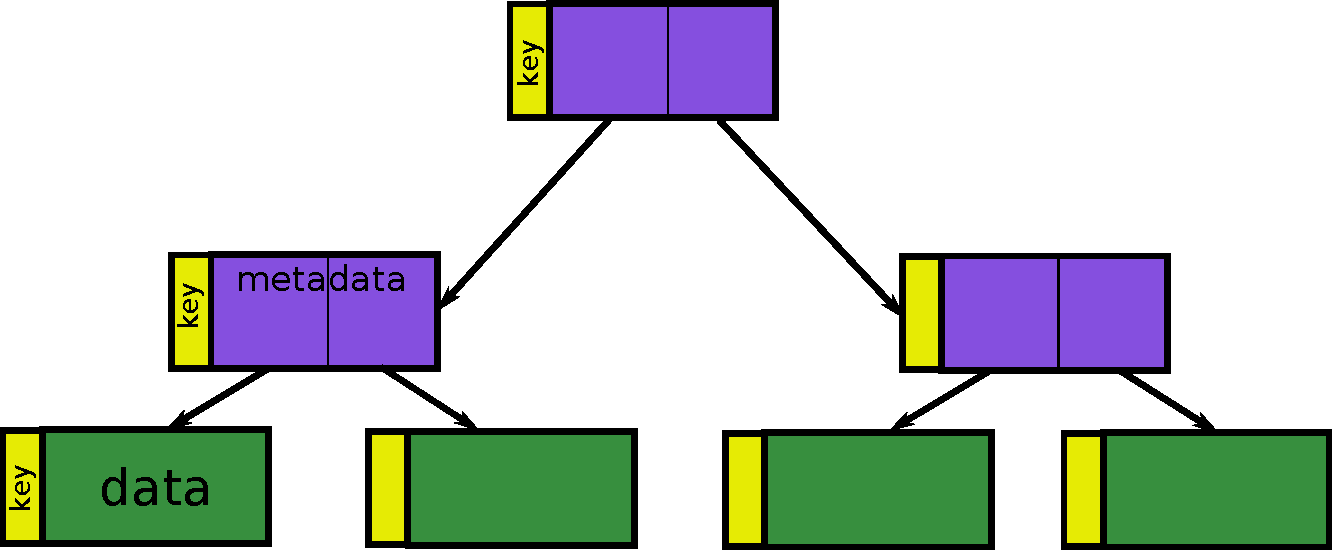
\includegraphics[width=3in]{tree}
\caption{\label{fig:tree}Example of how data is chunked and stored inside a SMACHE cache.}
\end{center}
\end{figure}

\begin{figure*}[htb]
\begin{center}
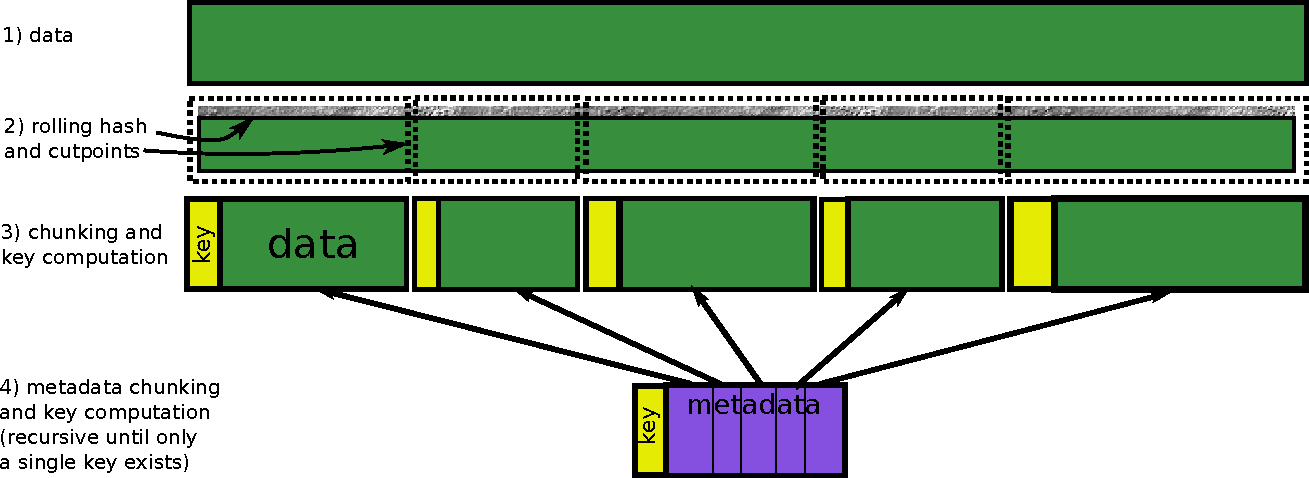
\includegraphics[width=5in]{algo}
\caption{\label{fig:algo} The algorithm used for storing data.}
\end{center}
\end{figure*}

Before detailing algorithms, we describe how data is represented by SMACHE.
All data in a SMACHE cache is uniquely identified by a single 16-byte hash
value.  This is known as the {\bf key}.  Complete files and small data chunks
are not differentiated.

All data chunks stored in a backend by SMACHE are less than 64Kb.  In order to
store data larger than this size, SMACHE automatically generates {\bf metadata}
chunks -- data chunks which contain lists of keys instead of actual data.  Data
is thus stored in a simple hierarchy, as illustrated in Figure~\ref{fig:tree}.
When retrieving the data associated with a metadata key, SMACHE transparently
traverses this tree and does not require the user of the library to have any
knowledge of metadata.  For example, the data contained in all four leaf nodes
in Figure~\ref{fig:tree} is uniquely identified by the key of the root node.
The user need only pass in this key, a length and an offset to in order to read
from the cache.  Access semantics are still effectively random, since each
metadata chunk may describe thousands of keys, not just two as depicted above
for simplicity.  In reality, the trees are very, very shallow.  Data would have
to be several terabytes before requiring more than a few levels.

Each block in a SMACHE cache has a reference count associated with it.  This
reference count is equal to the number of metadata blocks which refer to it
(note that metadata blocks can refer to other metadata blocks).  Keys that are
returned to the user of the library (e.g., when inserting a file) are given a
reference count of 1.  The library provides facilities for manipulating these
counts and automatically cleans up orphans.

\begin{figure}[htb]
\begin{center}
{\tiny {\bf {\tt
D21DB157405AA29E760B51B67B3C1477 M\_musculus/mm\_ref\_chr16.fa \\
76780C7295DD9144DCECC7D3FD238904 M\_musculus/mm\_ref\_chr11.fa \\
B3AFCF056DB76AF0CC8D459A1B208537 M\_musculus/mm\_ref\_chr10.fa \\
9E7D6046578135F121F2ABCB7E12156D M\_musculus/mm\_ref\_chr15.fa \\
$\vdots$ \\
C1E58171F9A4B0E9040D17D70CB90436 M\_musculus/mm\_ref\_chr06.fa \\
326AE42BCA5190BD884F1685AA5868CB M\_musculus/mm\_ref\_chr13.fa \\
49265721AC201C7EE44462008F4AF7BD M\_musculus/mm\_ref\_chr12.fa \\
9F1B6F170566BB9F053BF5765D8774EA M\_musculus/mm\_ref\_chr03.fa \\
}}}
\caption{\label{fig:index}An index for a SMACHE cache containing a Mouse genome.}
\end{center}
\end{figure}

Since all data is uniquely identified only by a hash, the python tools that
manipulate files (such as {\tt smachezip}) have a simple mechanism for
maintaining a mapping, known as the index, from a filename to a particular hash
(and set of metadata for that file, such as ownership, permissions and
modification times).  Figure~\ref{fig:index} shows a sample index file for a
cache containing a genome of the common mouse.  Such a mapping is similar to
the mapping from a filename to a disk block or inode number.

\subsection{Cache Insertion}

This Section describes the process of inserting data into a SMACHE cache, as
illustrated in Figure~\ref{fig:algo}.  The first step is to divide the data
into blocks using a block algorithm.  SMACHE supports using either Rabin-Karp
hashes with a specified mean block size as described in
Section~\ref{sec:insight} or fixed-size chunks.  Once the data is divided into
blocks, a key for each block is computing using an MD5 cryptographic hash.
Before insertion, each data block is compressed using a simple algorithm based
on Huffman coding; blocks are not compressed if there are no savings.  This
algorithm is better suited than a dictionary-based approach such as Lempel-Ziv,
since the blocks are generally quite small.  The compression aims only to save
space when data consists of all readable ASCII characters, for example.
Finally, a sequence of all keys describing the data is generated and this data
is recursively inserted to the cache.  When a single key may be used to
describe the data, this key is returned to the user.  The python tools use this
single key as the identifier for the file in the index.

\section{Evaluation}
\label{sec:evaluation}

We evaluate the disk usage of SMACHE compared to uncompressed data and data
that has been compressed with {\tt gzip}.  Note that we do not generally expect
to perform better than {\tt gzip}, since SMACHE is able to provide random
access semantics; the inability to access random at arbitrary positions within
the stream makes {\tt gzip} inappropriate for caching.

We break down the disk usage of SMACHE into four components.  First, there is
the {\bf data} itself.  This is space occupied by data from the original
stream, possibly slightly compressed as described in
Section~\ref{sec:implementation} Second, there are {\bf keys}; this is the
amount of data used to store all keys for data and metadata.  Third, there is
overhead associated with the storage of the {\bf metadata} itself.  Recall, the
metadata consists of lists of the keys that make up a chunk of large data.
Metadata chunks may be shared in the same way regular data chunks are shared.
Finally, there is overhead used by the database backend, referred to as {\bf DB
overhead}.  This overhead is related to data management structures employed by
the database on disk, and in a real system could be reduced enormously and
nearly eliminated (and our data management requirements are very simple).  As
described above, our implementation uses BekerleyDB~\cite{berkeleydb} to store
data, which demonstrated significant data overhead.

In this Section, we first test SMACHE on simple synthetic data to validate our
algorithms and provide a frame of reference.  Then, we evaluate its performance
on a set of biological data, consisting of a few complete genomes.  Finally, we
test its performance in storing VM images.

\subsection{Synthetic Data}

In order to establish that SMACHE does it what claims, we first choose a simple
set of synthetic benchmarks to cache.  We used {\tt smachezip} to compress one
megabyte of all zeros, one megabyte of random data (uncompressable), and the
same random data concatenated with a slightly modified copy of itself.

\begin{figure*}[htb]
\begin{center}
\subfigure[Zeros]
{
    \includegraphics[width=2.25in]{../test/sanity/077effb59e9d5fcfabca678cf6da604c-rabin-512-comparison}
}\hspace{-0.25in}
\subfigure[Random]
{
    \includegraphics[width=2.25in]{../test/sanity/7ddf32e17a6ac5ce04a8ecbf782ca509-rabin-512-comparison}
}\hspace{-0.25in}
\subfigure[Near-Duplicate Random]
{
    \includegraphics[width=2.25in]{../test/sanity/0573c34a9b45a255db3283bd05f25265-rabin-512-comparison}
}
\caption{\label{fig:synthetic}The performance of SMACHE on three simple synthetic data sets.}
\end{center}
\end{figure*}

Figure~\ref{fig:synthetic} shows the performance of SMACHE on these three data
sets relative to the original (uncompressed) data and data compressed with {\tt
gzip}.  The zero data is clearly compressed by both {\tt gzip} and SMACHE,
since all blocks are common, although SMACHE imposes slightly more overhead.
The random data is not compressed by either SMACHE or {\tt gzip}, since there
is very little self-similarity or compressability.  We can see here that the
overhead imposed by SMACHE itself is minimal -- primarily it is from the
database backend.  This overhead is easily removable by using a more
appropriate backend, we are not concerned with this aspect for this
implementation.

SMACHE achieves expected good performance on the duplicated random data set.
Discounting unnecessary database overhead, it handily beats the uncompressed
version and {\tt gzip}, since the data set demonstrates significant
self-similarity.  The amount of stored data is marginally more than half the
original size of the random data, as expected.  Note that this also
demonstrates the benefits of a content-sensitive block algorithm, since a
fixed-size block algorithm would not see repeated blocks due to the small
modification of the random data.

\subsection{Biological Data}

We evaluated the performance of SMACHE in storing biological data by caching
several complete genomes.  Each genome was several gigabytes in size. It is
difficult to know exactly what kinds of biological data will be commonly used
together by computational biologists, which is why SMACHE was designed as a
general-purpose mechanism.  We feel that storing related genomes is a
reasonable proof-of-concept approach. 

For all biological data, we use a block algorithm of Rabin-Harp rolling hashes
with a mean blocksize of 512 bytes.  Although using different blocksizes and
parameters for this algorithm yields interesting results, we found 512 bytes to
give reasonable performance and omit further analysis for the sake of brevity.

\subsubsection*{Single Genome}

To evaluate the self-similarity of a basic biological data set, we created a
cache consisting of the FASTA formatted files compromising the genome of the
common mouse.

\begin{figure*}
\begin{center}
\subfigure[Comparison]
{
\includegraphics[width=3in]{../test/bio/b491e5700331389ab45c50c0c2180d65-rabin-512-comparison}
\label{fig:biocomparison}
}
\subfigure[Compression]
{
\includegraphics[width=3in]{../test/bio/b491e5700331389ab45c50c0c2180d65-rabin-512-compression}
\label{fig:biocompression}
}
\subfigure[Data Reference Count Histogram]
{
\includegraphics[width=3in]{../test/bio/b491e5700331389ab45c50c0c2180d65-rabin-512-datahisto}
\label{fig:biodatarefs}
}
\subfigure[Metadata Reference Count Histogram]
{
\includegraphics[width=3in]{../test/bio/b491e5700331389ab45c50c0c2180d65-rabin-512-metahisto}
\label{fig:biometarefs}
}
\caption{Caching the complete genome of the common mouse.}
\end{center}
\end{figure*}

We see in Figure~\ref{fig:biocomparison} that SMACHE achieves reasonable
performance on the mouse genome.  However, the vast majority of this
performance is due to the level of compression achieved.  As shown in
Figure~\ref{fig:biocompression}, approximately 90\% of data blocks are
compressed, and a overall compression ratio of just above 50\% is achieved.
Although the optimal compression ratio for biological data is 25\% or below,
the FASTA files do contain other information and the compression algorithms
used are completely general-purpose.

Figure~\ref{fig:biodatarefs} shows that although there are several blocks that
were are repeated over 60 times, the majority of blocks appear only once in the
genome.  For example, over one million blocks were unique, whereas
approximately 10 thousand blocks were repeated twice.
Figure~\ref{fig:biometarefs} shows similarly that few sequences of blocks
(metadata blocks) were repeated.  This is expected, since relatively few blocks
were repeated.  Although we saw a single metadata block repeated eight times,
we expect that this is equivalent to a zero page (perhaps missing genomic data
or a long repeat in the genome).

\subsubsection*{Related Genomes}

We combined the complete mouse genome and complete human genome into a single
cache using {\tt smachezip} in order to evaluate the performance of the system
on related biological data.  Since the mouse and humans are both advanced
mammals, we expect to see significant sharing.

\begin{figure}[h]
\begin{center}
\subfigure[Comparison]
{
\includegraphics[width=3in]{../test/bio/aba44ef1ed1c9d294d37d3068c12806c-rabin-512-comparison}
\label{fig:relbiocomparison}
}
\end{center}
\begin{center}
\subfigure[Metadata Reference Count Histogram]
{
\includegraphics[width=3in]{../test/bio/aba44ef1ed1c9d294d37d3068c12806c-rabin-512-metahisto}
\label{fig:relbiometarefs}
}
\caption{Caching the complete mouse genome and complete human genome.}
\end{center}
\end{figure}

Figure~\ref{fig:relbiocomparison} shows that the performance of SMACHE is
similar to the case of a single genome.  Relative performance to {\tt gzip} was
only marginally better. Most of the gains come from compression as opposed to
sharing.  We expect that this is due to a large number of tiny differences
spread through the genomes that made exact block matches rarer than we would
have liked.

Although, interestingly we did see some small amount of sharing between the
genomes.  For example, Figure~\ref{fig:relbiometarefs} shows a histogram of the
reference counts for the metadata blocks.  The fact that these are
significantly higher indicates one of two things: humans have a lot of internal
genomic repetition of long sequences or there was sharing of a few long
sequences between humans and mice.  We feel it was likely a combination of the
two.

\subsubsection*{Multiple Genomes}

Finally, we tested performance of SMACHE when caching a larger set of genomes.
Due to the size of the data, we limited ourselves to four animals: the common
mouse, human, dog and chicken.

We found that the performance of SMACHE related to {\tt gzip} was similar to
the case of related genomes and omit graphs for that reason.  Again, we expect
that a very large number of tiny differences made exact block matches
difficult.  It may be worth exploring smaller block sizes, differencing
algorithms and fuzzy block matches for genomic data.  Unfortunately, a
Rabin-Karp-based block algorithm with a mean size of 512 bytes did not produce
the level of similarity that we expected.

\subsection{Virtual Machine Images}

For all VM image data, we use a fixed size block of 512 bytes.  This is
equivalent to the block size of the virtual disk and will allow us to
capitalize on the frequency of zeroed blocks, among other things.

\subsubsection*{Single Virtual Machine Image}

To establish a baseline, we downloaded a Debian VM image from {\tt
jailtime.org} and created a cache containing this image using the {\tt
smachezip} tool.

\begin{figure*}
\begin{center}
\subfigure[Comparison]
{
\includegraphics[width=3in]{../test/images/2d5bac171197ad549e012b332cbd8d97-fixed-comparison}
\label{fig:vmcomparison}
}
\subfigure[Compression]
{
\includegraphics[width=3in]{../test/images/2d5bac171197ad549e012b332cbd8d97-fixed-compression}
\label{fig:vmcompression}
}
\subfigure[Data Reference Count Histogram]
{
\includegraphics[width=3in]{../test/images/2d5bac171197ad549e012b332cbd8d97-fixed-datahisto}
\label{fig:vmdatarefs}
}
\subfigure[Metadata Reference Count Histogram]
{
\includegraphics[width=3in]{../test/images/2d5bac171197ad549e012b332cbd8d97-fixed-metahisto}
\label{fig:vmmetadatarefs}
}
\caption{Caching a single Debian Virtual Machine image.}
\end{center}
\end{figure*}

SMACHE stores a single VM image very efficiently, coming very close to {\tt
gzip} in terms of space efficiency.  We find that it is only tens of megabytes
above {\tt gzip} when the unnecessary overhead associated with the database is
discounted.

For non-redundant data stored, we achieve a compression ratio of about 75\%.
This poor ratio is unsurprising, as the data in a VM image is generally binary
and SMACHE compression can operate on only small blocks.  With this amount of
data, there is rarely enough information to achieve reasonable compression with
fairly uniformly distributed binary data.  Figure~\ref{fig:vmcompression} shows
the percentage of blocks that were compressed.

Figure~\ref{fig:vmdatarefs} shows a surprising number of blocks that have 10,
20 and even 50 references.  These are likely patterns such as compiler-inserted
stubs (e.g., as crt0.o), shared library hooks and trampolines, template code,
and filesystem structures such as blank inodes.  The majority of the savings,
however, were likely due to a few highly repeated blocks (such as a zero
block).  We see a single block with a reference count of over 800.

Figure~\ref{fig:vmmetadatarefs} shows that longer sequences are rarely
repeated.  This is sensible, since the layout of the filesystem will largely be
block-based, and not as a complete sequence as in the biological example.

\subsubsection*{Related Virtual Machine Images}

We explore the effectiveness of SMACHE storing related VM images by creating a
cache with two VM images: the unmodified image from the case above, and the
same image after an upgrade and mild usage.  To derive the modified image, the
unmodified Debian image was first copied and upgraded through the standard {\tt
apt-get upgrade} procedure.  The upgrade affected several hundred packages (the
majority of the software found on the image).  Then, the modified image was
used for development of SMACHE over the course of several hours, additionally
requiring that several extra packages be installed.

\begin{figure}
\begin{center}
\includegraphics[width=3in]{../test/images/e0fc81e2aa971046022f1451918d4c01-fixed-comparison}
\caption{\label{fig:relvmcomparison}Caching two related Virtual Machine images.}
\end{center}
\end{figure}

Figure~\ref{fig:relvmcomparison} shows the performance of SMACHE compared to a flat
cache and {\tt gzip}.  Surprisingly, once overhead from the database is
discounted, SMACHE stores data {\bf more efficiently} than even {\tt gzip},
while still giving random access semantics.  We see this because a large number
of blocks are shared across the two images, since the percentage of blocks with
references greater than one is significantly higher than in the case of a
single VM image; the histogram is not shown here since visibly this is not
obvious.  This is a remarkably result, since non-trivial changes were introduced
to the second VM image.  Most of the savings are from sharing between the
images; compression helps only marginally, as in the case of a single VM image.

We can conclude that SMACHE would be very effective at storing a large number
of related VM images.  In compute clouds this is likely to be a very common
scenario; an approach such as SMACHE appears very promising.

\subsubsection*{Different Distributions}

We additionally tested the efficiency of SMACHE in storing completely unrelated
VM images.  In addition to the basic Debian VM image described above, we cached
a Fedora Core 9 image also downloaded from {\tt jailtime.org}.

\begin{figure}
\begin{center}
\includegraphics[width=3in]{../test/images/c28bddb249ce1bb2c1d1979605bcc6a5-fixed-comparison}
\caption{\label{fig:difvmcomparison}Caching two unrelated Virtual Machine images.}
\end{center}
\end{figure}

Figure~\ref{fig:difvmcomparison} shows less impressive performance than caching
related VM images.  For the most part, we see that the space taken is the sum
of storing two independent images.  However, this is not unreasonable as these
images contain completely different software packages with completely different
versions.  All configuration files and metadata within the image are also
different.  We find that sharing between VM images is not as significant in
this case of related VM images, since relatively fewer blocks have more than
one reference count.

As in the case of a single image, we see significant savings realized through a
couple of highly repeated blocks at approximately 2600 and 3000 references
each.  Compression also helps here, achieving a ratio of approximately 50\%.

We can conclude that although SMACHE does not see significant savings for
unrelated images, there is little disadvantage here.  We still realize savings
through internal self-similarity and compression of individual blocks.

\section{Conclusion}
\label{sec:conclusion}

Cloud and cluster computing is an important factor in tackling ``big data''
problems.  Systems support for distributed programming paradigms such as
Map-Reduce and SnowFlock are still young.  SMACHE implements a general-purpose
space-efficient cache which services can use to store both biological or
scientific data as well as program data.  This cache represents an important
building block for scalable storage systems in cluster computing.

In particular, we saw very promising results for storing related VM images,
actually beating standard compression techniques while still providing random
access semantics.  Results storing biological data sets were not as stunning,
however we feel that there is room for improvement by exploring better block
algorithms, performing near blocks matches and storing differential data.  In
any case, SMACHE handily beat out the flat caching mechanism, likely making it
an more appropriate choice than either no compression or standard compression
techniques in most scenarios.

\bibliographystyle{abbrv}
\bibliography{bio}

\end{document}
